\chapter{The Basic Transport Equations}
\label{sec:Theory_Chapter}

The equations used in CFAST take the form of an initial value problem for a system of ordinary differential equations. These equations are derived from the conservation laws of mass and energy (equivalently the first law of thermodynamics) and the ideal gas law. These equations predict as functions of time quantities such as pressure, layer height and temperatures given the gains and losses of mass and energy in the two layers. The assumption of a zone model is that properties such as temperature can be approximated throughout a control volume by an average value. Many formulations based upon these assumptions can be derived. Though equivalent mathematically, these formulations differ in their numerical solution.

The exchange of mass and enthalpy between zones is due to physical phenomena such as fire plumes, natural and forced ventilation, convective and radiative heat transfer, and so on. For example, a vent exchanges mass and enthalpy between zones in connected rooms, a fire plume typically adds heat to the upper layer and transfers entrained mass and enthalpy from the lower to the upper layer, and convection transfers enthalpy from the gas layers to the surrounding walls.


 It is assumed that each compartment is divided into two control volumes, a relatively hot upper layer and a relatively cool lower layer, as illustrated in Fig.~\ref{fig:Control_Volumes}. The gas temperature and density are assumed constant in each layer. The compartment as a whole is assumed to have a single value of pressure, $P$. It is also assumed that all thermodynamic parameters are constant. The specific heat at constant volume and at constant pressure, $c_v$ and $c_p$, the universal gas constant, $R$, and the ratio of specific heats, $\gamma$, are related by $\gamma = c_p / c_v$ and $R = c_p- c_v$.  For ambient air, $c_p \approx 1$~kJ/(kg $\cdot$ K) and $\gamma = 1.4$.
\begin{figure}[h]
\begin{center}
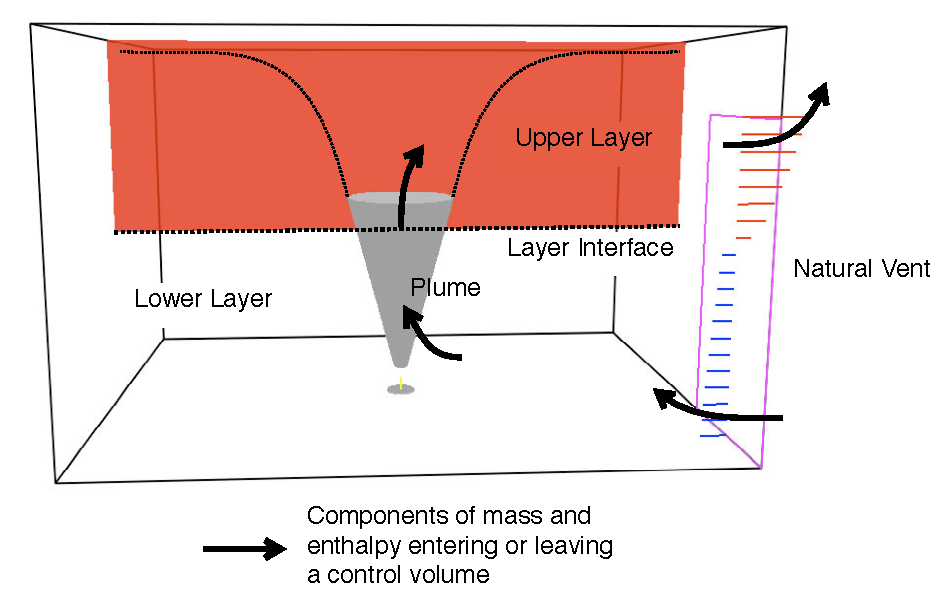
\includegraphics[width=\textwidth]{FIGURES/Theory/Control_Volumes}\\
\end{center}
\caption{Schematic of control volumes in a two-layer zone model.}
 \label{fig:Control_Volumes}
\end{figure}
Conservation of mass in each layer, $\dot m_i$, is expressed
\be
   \dbydt{m_i} = \dot m_i  \label{mass_con}
\ee
Conservation of energy takes the form of the first law of thermodynamics, which states that the rate of increase of internal energy plus the rate at which the layer does work by expansion is equal to the rate at which enthalpy is added to the gas:
\be
   \dbydt{(c_v m_i T_i)} +  P \dbydt{V_i} =  \dot h_i \label{eq:first_law}
\ee
The enthalpy source term, $\dot h_i$, consists of the fire's heat release rate, conduction losses to walls, and radiation exchange. The layer temperature and mass are related to the layer volume and compartment pressure via the ideal gas law:
\be
  P \, V_i = m_i \, R \, T_i \label{EoS}
\ee
A system of ordinary differential equations for the compartment pressure, upper layer volume, and layer temperatures can be derived from these three basic principles:
\begin{eqnarray}
\dbydt{P} &=& \frac{{\gamma-1}}{{V}} \left( \dhl + \dhu \right)  \\[.1in]
\dbydt{\Vu} &=& \frac{1}{P \gamma} \left( (\gamma-1) \, \dhu - \Vu \dbydt{P} \right) \\[.1in]
\dbydt{\Tu} &=& \frac{1}{c_p \, m_{\rm u}} \left( \dhu - c_p \, \dmau \, \Tu + \Vu \dbydt{P} \right) \\[.1in]
\dbydt{\Tl} &=& \frac{1}{c_p \, m_{\rm l}} \left( \dhl - c_p \, \dmau \, \Tl + \Vl \dbydt{P} \right)
\end{eqnarray}
As discussed in Refs.~\cite{Forney:1994} and \cite{Rehm:1992}, these equations are stiff, meaning that the pressure adjusts to changing conditions more quickly than the other variables. Runge-Kutta methods or predictor-corrector methods such as Adams-Bashforth require prohibitively small time steps in order to track the short time scale phenomena (pressure in our case). Methods that calculate the Jacobian (or at least approximate it) have a much larger stability region for stiff problems and are thus more successful at their solution.





\chapter{The Fire Plume}
\label{sec:TheFire}

Fires in CFAST are specified by the user in terms of a time-dependent heat release rate (HRR), an effective fuel molecule, and the yields of the products of incomplete combustion like soot and CO. Fires can be specified in multiple compartments and are treated as totally separate entities, with no interaction of the plumes. These fires are generally referred to as ``objects'' and can be ignited at a prescribed time, temperature or heat flux.

CFAST does not include a pyrolysis model to {\em predict}, as opposed to specify, the growth and spread of the fire. Rather, pyrolysis rates for each fire are prescribed by the user. While this approach does not directly account for increased pyrolysis due to radiative feedback from the flame or compartment, in theory these effects could be prescribed by the user. In an actual fire, this is an important consideration, and the specification used should consider the experimental conditions as closely as possible.

\section{Combustion Chemistry}

 The HRR of the fire is specified by the user, but it may be constrained by the availability of oxygen in the compartment. The combustion of a hydrocarbon fuel is described by the following single-step reaction:
\begin{eqnarray}
   \mathrm{C_{n_\C}H_{n_H}O_{n_O}N_{n_N}Cl_{n_{Cl}}} &+&  \nu_\OTWO \, \mathrm{O_2}  \rightarrow  \nonumber \\[.1in]
   \nu_\COTWO \, \mathrm{CO_2} &+& \nu_\HTWOO \, \mathrm{H_2O} \; + \; \nu_\CO \, \mathrm{CO} \; + \; \nu_\So \, \mathrm{Soot} \; + \; \nu_\HCl \mathrm{HCl} \; + \; \nu_\HCN \mathrm{HCN} \label{stoich}
\end{eqnarray}
The user specifies the composition of the fuel molecule and the yields of soot and CO, $y_\So$ and $y_\CO$, which are related to their stoichiometric coefficients as follows:
\begin{eqnarray}
   \nu_\So &=& \frac{M_\F}{M_\So} \; y_\So \label{soot_yield} \\[.1in]
   \nu_\CO &=& \frac{M_\F}{M_\CO} \; y_\CO \label{CO_yield}
\end{eqnarray}
Under the assumption that all of the nitrogen and chlorine in the fuel are converted to HCN and HCl, the other stoichiometric coefficients are:
\begin{eqnarray}
  \nu_\COTWO &=& \mathrm{n_\C} - \brackets{\nu_\CO + \nu_\HCN + \nu_\So} \\[.1in]
  \nu_\HTWOO &=& \frac{\mathrm{n_\Hy} - \brackets{\nu_\HCl + \nu_\HCN}}{2} \\[.1in]
  \nu_\OTWO  &=& \nu_\COTWO + \frac{\nu_\HTWOO + \nu_\CO - \mathrm{n_\Oh}}{2} \label{Oxygen_yield} \\[.1in]
  \nu_\HCl   &=& \mathrm{n_{Cl}} \\[.1in]
  \nu_\HCN   &=& \mathrm{n_{N}}
\end{eqnarray}
Note that the nitrogen in the air acts only as a diluent. The yields of hydrogen cyanide and hydrogen chloride are based solely on the composition of the fuel molecule. Finally, a user-specified trace species can be specified to follow the transport that results from fire-induced flow for an arbitrary species. This may be of particular interest for radiological releases \cite{Jones:2008}, but may be useful for any trace amounts released by a fire.

\section{Heat Release Rate}

As fuel and oxygen are consumed, heat is released and various products of combustion are formed. The heat is released as radiation and convected enthalpy:
\begin{eqnarray}
   \dQr &=& \chi_{\rm r} \, \dQ \\[.1in]
   \dQc &=& (1-\chi_{\rm r}) \, \dQ
\end{eqnarray}
where, $\chi_{\rm r}$ is the fraction  of the fire's heat release rate given off as radiation. The default value to 0.30~\cite{Drysdale:1985}.

While it is convenient for the user to directly specify the heat release rate of the fire, it is actually the pyrolysis rate of fuel, $\dmf$, that is specified:
\be
   \dmf = \frac{\dQ}{\Dh}
\ee
where $\Dh$ is the heat of combustion. In the event that the HRR is constrained by the availability of oxygen, the pyrolysis rate does not change, but the HRR becomes:
\be
   \dQ = \min \Big( \dmf \, \Dh \, , \, \dme \, Y_\OTWO \, C_{\rm LOL} \, \DhO \Big)
\ee
where $\dme$ is the entrainment rate, $Y_\OTWO$ is the mass fraction of oxygen in the layer containing the fire, $\DhO$ is the heat of combustion based on oxygen consumption\footnote{The heat of combustion based on oxygen consumption is taken to be 13.1~MJ/kg, representative of typical hydrocarbon fuels~\cite{Huggett:1980}.}, and $C_{\rm LOL}$ is the smoothing function ranging from 0 to 1:
\be
   C_{\rm LOL} = \frac{\tanh \Big( 800 (Y_\OTWO - Y_{\OTWO,{\rm l}}) - 4 \Big) + 1}{2}
\ee
The limiting oxygen mass fraction, $Y_{\OTWO,{\rm l}}$, is 0.1, by default.



\section{Plume Entrainment}

The mass entrainment of air, $\dme(z)$, into the plume at a height $z$ above the base of the fire is estimated using either McCaffrey's~\cite{McCaffrey:1983} or Heskestad's~\cite{Heskestad:1984} correlation. McCaffrey divides the flame/plume into three regions:
\be
   \frac{\dme(z)}{\dQ} = \left\{ \begin{array}{r@{\quad \quad}l}
   0.011 \brackets{\ZQf}^{0.566} &  0.00 \leq \brackets{\ZQf}<0.08 \\[.1in]
   0.026 \brackets{\ZQf}^{0.909} &  0.08 \leq \brackets{\ZQf}<0.20 \label{eq:McCaffreyPlume} \\[.1in]
   0.124 \brackets{\ZQf}^{1.895} &  0.20 \leq \brackets{\ZQf} \end{array} \right.
\ee
Heskestad analyzed both his own data \cite{Heskestad:1984} and that of Zukoski \cite{Zukoski:1981} to develop the correlation
\be
   \dme(z) = 0.071 \, \dQ_{\rm c}^{1/3} \; \brackets{z - z_0}^{5/3} \; \brackets{1 + 0.026 \, \dQ_{\rm c}^{2/3} \, \brackets{z-z_0}^{-5/3}}
\ee
where $z_0$ is a virtual origin for the fire plume defined as
\be
  z_0/D = -1.02 + 0.083 \dQ^{2/5} / D
\ee
which is based on the total heat release rate of the fire, $\dQ$.  Both correlations provide similar results in CFAST calculations.

In CFAST, there is a constraint on the mass entrainment rate because the plume can rise only so high for a given HRR.  Early in a fire, the plume may not have sufficient energy to reach the compartment ceiling. Therefore, a limit is placed on the entrainment rate. For the plume to be able to penetrate the hot upper layer, the density of the gas in the plume must be less than the density of the gas in the upper layer. This implies that the upper layer temperature must be less than the plume temperature:
\be
   \Tu < \Tp \approx \frac{ \dQc + \dme \, c_p \, \Tl }{ \dme \, c_p}
\ee
Rearranging terms yields a limit on the mass entrainment:
\be
   \dm_e < \frac{\dQc}{c_p (\Tu - \Tl)}
\ee


\section{Plume Centerline Temperature}

CFAST includes an empirical correlation of plume centerline gas temperature based on the work of Baum and McCaffrey~\cite{Baum:1989} with a modification by Evans~\cite{Evans:1984} to account for the presence of a hot gas layer. The correlation gives the excess temperature as a function of height above a fire, $z$, for the flaming, intermittent, and plume regions:
\be
   \frac{\Delta \Tp}{T_\infty} = \left\{ \begin{array}{l@{\quad \quad}l}
   2.91                   &  0.00 \leq z/D^* < 1.32  \\[.1in]
   3.81 \, (z/D^*)^{-1}   &  1.32 \leq z/D^* < 3.30 \\[.1in]
   8.41 \, (z/D^*)^{-5/3} &  3.30 \leq z/D^* \end{array} \right.
\ee
where
\be
  D^* = \left( \frac{\dQ}{\rho_\infty c_p T_\infty \sqrt{g}} \right)^{2/5}
\ee
Figure~\ref{fig:Plume_Temp} shows the correlation. When a hot layer forms, the correlation must be modified since the plume now includes added enthalpy due to the entrainment of hot layer gases. Evans~\cite{Evans:1984} defines a virtual source and heat release rate to extend the plume into the upper layer. Evans' method defines the strength and location of the substitute source with respect to the interface between the upper and lower layers by

\begin{figure}
\begin{center}
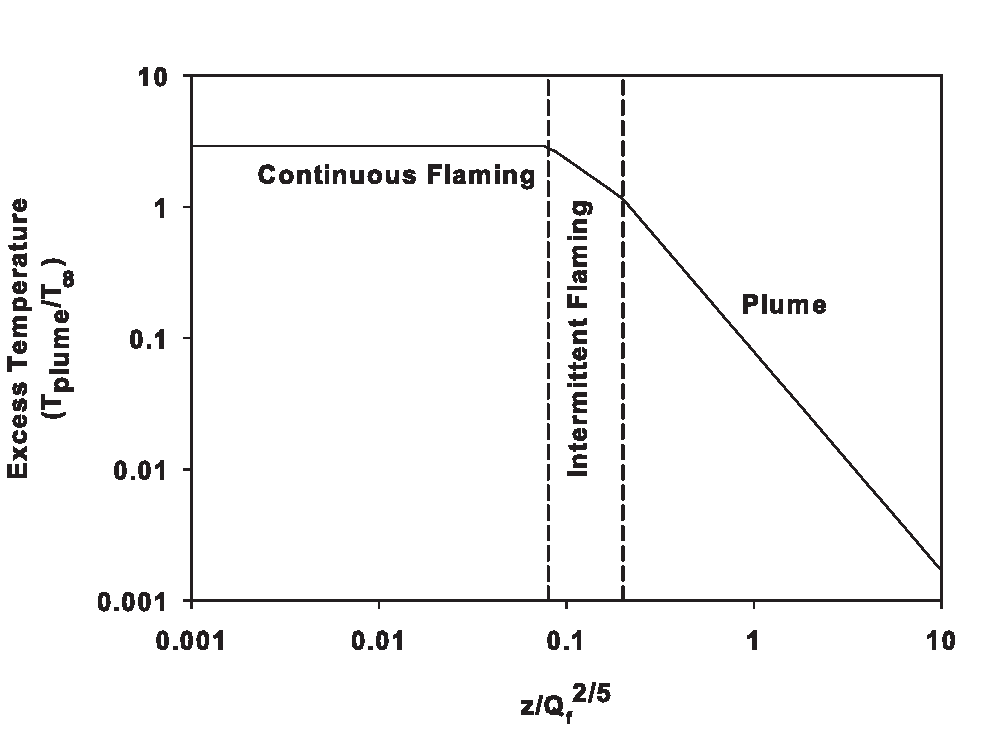
\includegraphics[width=4.0in]{FIGURES/Theory/Plume_Temperature}\\
\end{center}
\caption{Excess plume centerline temperature from Baum and McCaffrey correlation.}
 \label{fig:Plume_Temp}
\end{figure}

\be Q_{I,2}^* = \brackets{\frac{1 + C_T {Q_{I,1}^*}^{2/3}}{\xi C_T} - \frac{1}{C_T}}^{3/2} \ee

\be Z_{I,2} = \brackets{\frac{\xi Q_{I,1}^* C_T}{{Q_{I,2}^*}^{1/3}\brackets{\brackets{\xi - 1}\brackets{\beta^2 + 1}+ \x1 C_T {Q_{I,2}^*}^{2/3}}}}^{2/5} Z_{I,1}  \ee

\be Q_{I,1}^* = \frac{Q_{f,C}}{\rho_\infty c_p T_\infty \sqrt{g} Z_{I,1}^{5/2}}  \ee
where $Z_{I,1}$ is the distance from the fire to the interface between the upper and lower gas layers, $Z_{I,2}$ is the distance from the virtual source to the layer interface, $\xi$ is the ratio of the upper to lower layer temperature, $\beta$ is an experimentally determined constant \cite{Zukoski:1981} ($\beta^2 = 0.913$), and $C_T = 9.115$.  The effective source strength and distance between the virtual source and target position is given by

\be Q_{f,C,eff} = Q_{I,2}^* \rho_\infty c_{p\infty} T_\infty \sqrt{g} Z_{I,2}^{5/2}  \ee

\be z_{eff} = z - Z_{I,1} + Z_{I,2} \ee
(see Fig.~\ref{fig:Plume_Temp_Notation}). The new values of the fire source and  target location are then used in the standard plume correlation where the ambient conditions are now those of the upper layer.
\begin{figure}
\begin{center}
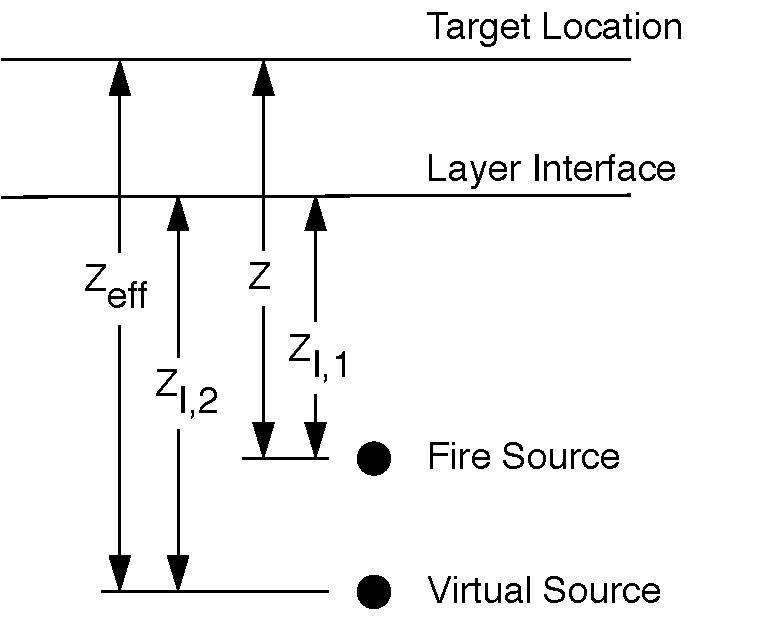
\includegraphics[width=4.0in]{FIGURES/Theory/Plume_Temp_Notation}\\
\end{center}
\caption{Geometry for plume centerline temperature calculation.}
 \label{fig:Plume_Temp_Notation}
\end{figure}

\section{Flame Height}
\label{sec:firemassbalance}


CFAST includes a calculation of average flame height based on the work of Heskestad~\cite{Heskestad:2002}. Valid for a wide range of hydrocarbon and gaseous fuels, the correlation is given by
\be
   H = -1.02 D + 0.235 \brackets{\frac{Q_f}{1000}}^{2/5}
\ee
where $H$ is the average flame height (m), $D$ the diameter of the fire (m), and $\dQ$ is the total heat release rate (kW). The mean flame height is defined as the distance from the fuel source to the top of the visible flame where the intermittency is 0.5.  A flame intermittency of 0.5 means that the visible flame is above the mean 50 \% of the time and below the mean 50~\% of the time.  This average flame height is  included in the printed output from CFAST.







\chapter{Ventilation}

CFAST models three types of vent flow: natural flow through vertical vents (such as doors or windows),  natural flow through horizontal vents (such as ceiling holes or hatches), and forced flow via mechanical ventilation. Forced flow can occur through either vertical or horizontal vents.

Atmospheric pressure is about 100~kPa. Fires produce pressure changes from 1~Pa to 1~kPa and mechanical ventilation systems typically involve pressure differentials of about 1~Pa to 100~Pa.  The pressure variables are solved to a higher accuracy than other solution variables because of the subtraction (with resulting loss of precision) needed to calculate vent flows from pressure differences.


\section{Vertically-Oriented Vents (Doors and Windows)}

Natural flow through windows and doors is governed by the pressure difference across the opening.  A momentum equation for the zone boundaries is not solved directly.  Instead momentum transfer at the zone boundaries is included by using Bernoulli's equation augmented for restricted openings with an orifice coefficient~\cite{Quintiere:1984, Steckler_Coefficients}.

The mass flow through a vertical opening is calculated by dividing the vertical extent of the opening into discrete segments, each of which is bounded by either the top or bottom of the door or window, the zone interface of either compartment, or the neutral plane, which is where the velocity changes direction. In this way, the vent opening is partitioned into at most six sections.

Let $z=b$ and $z=t$ denote the height of the bottom and top of the segment, and $\Delta P_b$ and $\Delta P_t$ denote the pressure differences at those heights.  Because the segment is either completely above or completely below the neutral plane, the two pressure differences will have the same sign. The mass flow through the segment can then be computed by integrating from $b$ to $t$:
\begin{eqnarray}
\dm &=& \int_b^t C \sqrt{2 \rho \, \Delta P(z)} \, w \, dz  \\[.1in]
    &=& C\sqrt{2\rho} \, w \int_b^t\sqrt{\frac{|(t-z) \, \Delta P_b + (z-b) \, \Delta P_t|}{t-b}} \; dz \\[.1in]
    &=& \frac{2}{3} \, C \sqrt{2\rho} \, w \, (t-b)\frac{|\Delta P_t|^{3/2}-|\Delta P_b|^{3/2}}{|\Delta P_t|-|\Delta P_b|}
\label{eq:massflowone}
\end{eqnarray}
Here, $C$ is the orifice coefficient taken to be 0.7~\cite{Steckler_Coefficients}, $\rho$ is the gas density of the upwind compartment, and $\Delta P(z)$ is the pressure across the interface at elevation $z$. Note that the integral is evaluated from
\begin{eqnarray}
\int \sqrt{A+Bz} \, dz = \frac{2}{3B}(A+Bz)^{3/2}+\mbox{constant}
\end{eqnarray}
where $A=(|t\,\Delta P_t|-b\,|\Delta P_b|)/(t-b)$ and $B=(|\Delta P_t|-|\Delta P_b|)/(t-b)$.
Equation \ref{eq:massflowone} is sometimes written:
\be
   \dm = \frac{2}{3} C \sqrt{2 \rho} \, w \, (t-b)  \frac{|\Delta P_t|+\sqrt{|\Delta P_t \,\Delta P_b|}+|\Delta P_b|}{\sqrt{|\Delta P_t|}+\sqrt{|\Delta P_b|} }
\ee

The mass flows through the various vertical segments of the door or window are distributed into the upper and lower layers of the downstream compartment depending on the temperature of the stream. Consider the flow of gas from the upper layer of Compartment~1 entering the lower layer of Compartment~2 (see Fig.~\ref{fig:Flow_Patterns}).
\begin{figure}[t]
\begin{center}
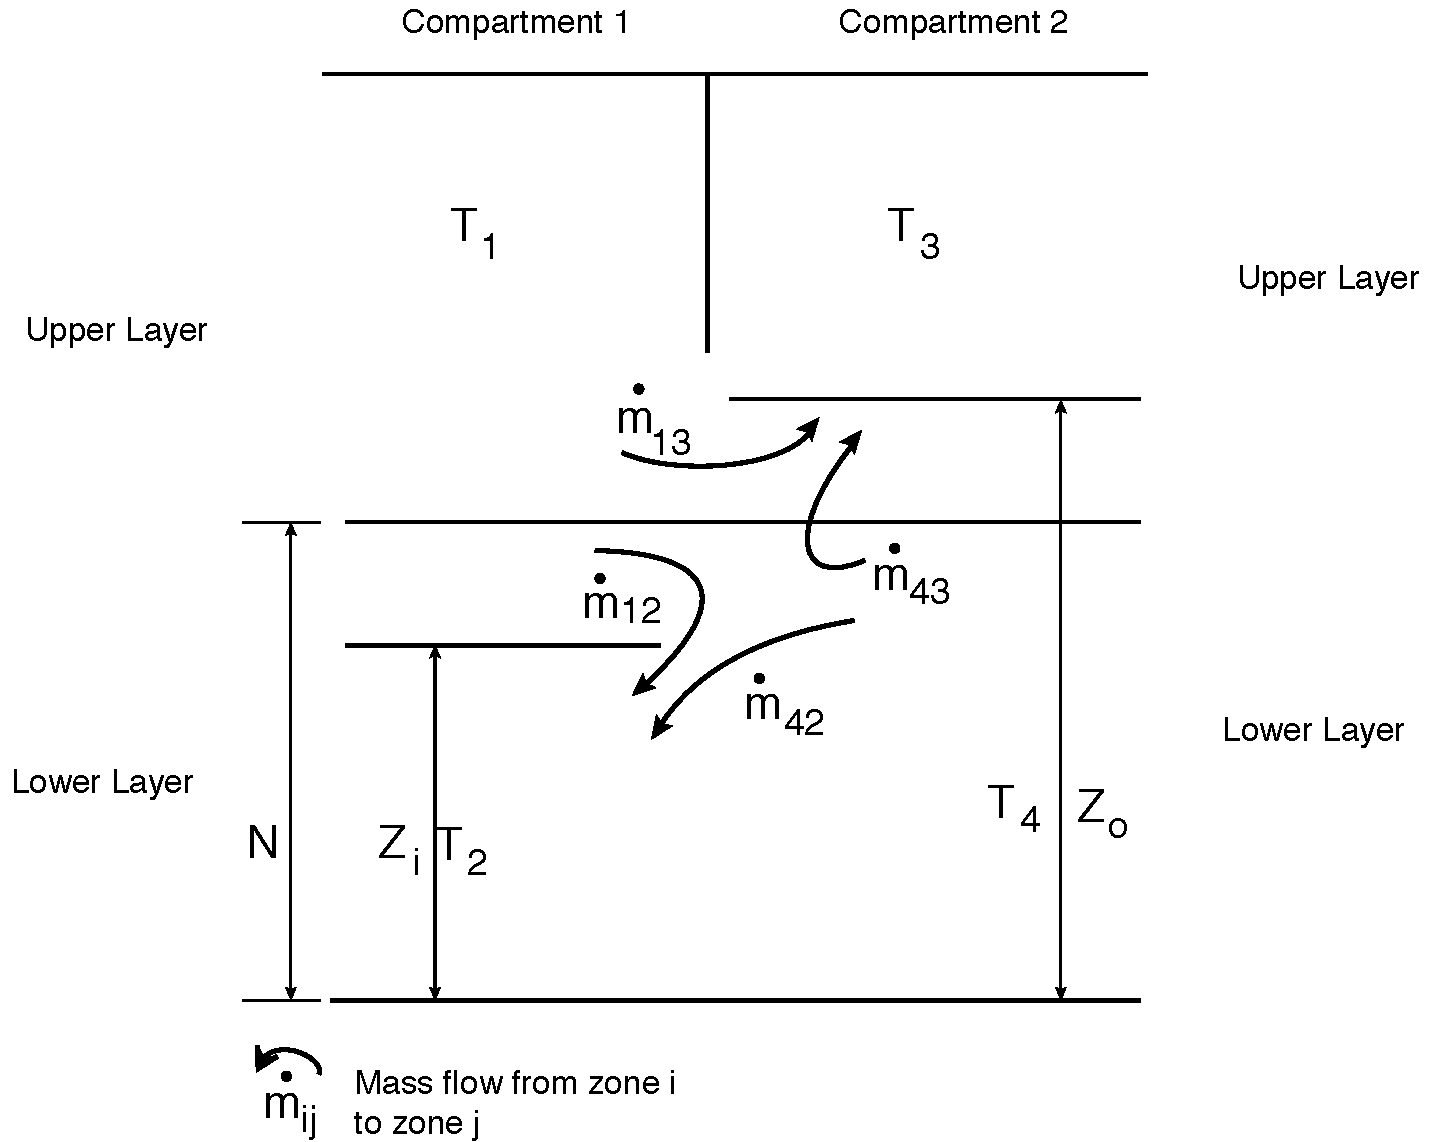
\includegraphics[width=5.0in]{FIGURES/Theory/Flow_Patterns}\\
\end{center}
\caption{Flow patterns and layer number conventions for horizontal flow through a vertical vent.}
 \label{fig:Flow_Patterns}
\end{figure}
The mass flow rate is denoted $\dm_{14}$, where the subscripts indicate the upstream and downstream layer indices, respectively. The enthalpy flow rate is:
\be
   \doh_{14} = c_p \brackets{T_1-T_4} \dm_{14}
\ee
Assuming that $T_4 < T_1 < T_3$, this energy will be distributed between the compartments two layers. The distribution is based on the relative difference in temperature between the incoming gas stream and the layer temperatures. If $T_1$ is close to $T_3$, most of the energy will go to the upper layer 3 in the form of a virtual plume. The effective heat release rate of this virtual plume is:
\be
   \dQ_{\rm eff} = \frac{T_1-T_4}{T_3-T_4} \; \doh_{14}
\ee
The mass entrainment rate into this virtual plume at the midpoint of the vertical segment, $\bar{z}$, is:
\be
   \dm_{\rm e,eff}(\bar{z}-z_0) = \frac{T_1-T_4}{T_3-T_4} \; \dm_{14}
\ee
The origin of the virtual plume, $z_0$, is deduced from McCaffrey's entrainment correlation, Eq.~\ref{eq:McCaffreyPlume}. That is, $\bar{z}-z_0$ is the height above the base of the virtual fire whose HRR is $\dQ_{\rm eff}$ where the mass entrainment rate is $\dm_{\rm e,eff}$.

The other type of mixing is much like an inverse plume and causes contamination of the lower layer.  It occurs when there is flow of the type $\dm_{42} > 0$.  The shear flow causes vortex shedding into the lower layer and thus some of the particulates end up in the lower layer.  The actual amount of mass or energy transferred is usually not large, but its effect can be large.  For example, even minute amounts of carbon can change the radiative properties of the gas layer, from negligible to something finite.  It changes the rate of radiation absorption significantly and invalidates the simplification of an ambient temperature lower layer.  This term is predicated on the Kelvin-Helmholz flow instability and requires shear flow between two separate fluids.  The mixing is enhanced for greater density differences between the two layers. However, the amount of mixing has never been well characterized. Quintiere et al. \cite{Quintiere:1984} discuss this phenomena for the case of crib fires in a single room, but their correlation does not yield good agreement with experimental data in the general case \cite{Quintiere:1981}.  In the CFAST model, it is assumed that the incoming cold plume behaves like the inverse of the usual door jet between adjacent hot layers; thus we have a descending plume.  The same equations are used to calculate this inverse plume as are used for the upright door mixing, above. It is possible that the entrainment is overestimated in this case, since buoyancy, which is the driving force, is not nearly as strong as for the usually upright plume.

\section{Horizontally-Oriented Vents (Floor and Ceiling Vents)}

Flow through a ceiling or floor vent is governed by both pressure and density differences. The simplest form is uni-directional flow driven primarily by a relatively large pressure difference. When the pressure difference is relatively small, the density difference, where hot gas underlies colder gas, can lead to bi-directional flow where the gas in the lower compartment rises into the upper compartment and {\em vice versa}.  This situation might arise in a real fire if the room of origin suddenly has a hole open up in the ceiling.

Cooper's algorithm~\cite{Cooper:1989, Cooper:1990, Cooper:1995} is used for computing mass flow through ceiling and floor vents:
\be
   \dm = 0.1 \brackets{\frac{g \, \Delta \rho \, A_{\rm v}^{5/2}}{\rho_{\rm avg}}} \brackets{1 - \frac{2 \, A_{\rm v}^2 \, \Delta P}{S^2 \, g \, \Delta \rho \, D^5}}
\ee
where $D = 2 \sqrt{A_{\rm v} / \pi}$ and $S$ is 0.754 for round or 0.942 for square openings, respectively. For each layer on either side of the vent, there are two values of the mass flow, $\dm_{\rm in}$ and $\dm_{\rm out}$. These terms are symmetric: the outgoing flow from one compartment is the incoming flow to the other. The corresponding enthalpy flows are determined from the relative size and temperature of the lower and upper layers:
\begin{eqnarray}
  \doh_{\rm in} &=& c_p \, \dmu \, \Tu + c_p \, \dml \, \Tl \\[0.1in]
  \dmu &=& \dm_{\rm in} \, \frac{\Vu}{V} \\[0.1in]
  \dml &=& \dm_{\rm in} \, \frac{\Vl}{V}
\end{eqnarray}
The mass and energy are then deposited into the upper or lower layer of the receiving compartment based on the effective temperature of the incoming flow relative to the upper and lower layers of the receiving compartment. If the temperature of the incoming flow is higher than the temperature of the lower layer, then the flow is deposited into the upper layer. This is similar to the idea of using a virtual plume for a doorway flow.


\section{Forced Flow}

CFAST models mechanical ventilation in terms of user-specified volume flows at various points in the compartment. The model does not include duct work or fan curves. These equations are high-order, non-linear and in some cases ill-posed, which caused a great deal of difficulty in reaching a numerical solution.

Figure~\ref{fig:Fans_and_Ducts}(a) depicts smoke exhaust via a fan at the top of an atrium, and Fig.~\ref{fig:Fans_and_Ducts}(b) illustrates a kitchen exhaust fan.  Cross ventilation, shown in Fig.~\ref{fig:Fans_and_Ducts}(c), is occasionally used without heating or cooling.  Generally systems that maintain comfort conditions have either one or two fans. Further information about these systems is presented in Klote and Milke~\cite{Klote:2002} and the American Society of Heating, Refrigerating and Air Conditioning Engineers (ASHRAE) \cite{ASHRAE:2001}.

\begin{figure}
\begin{center}
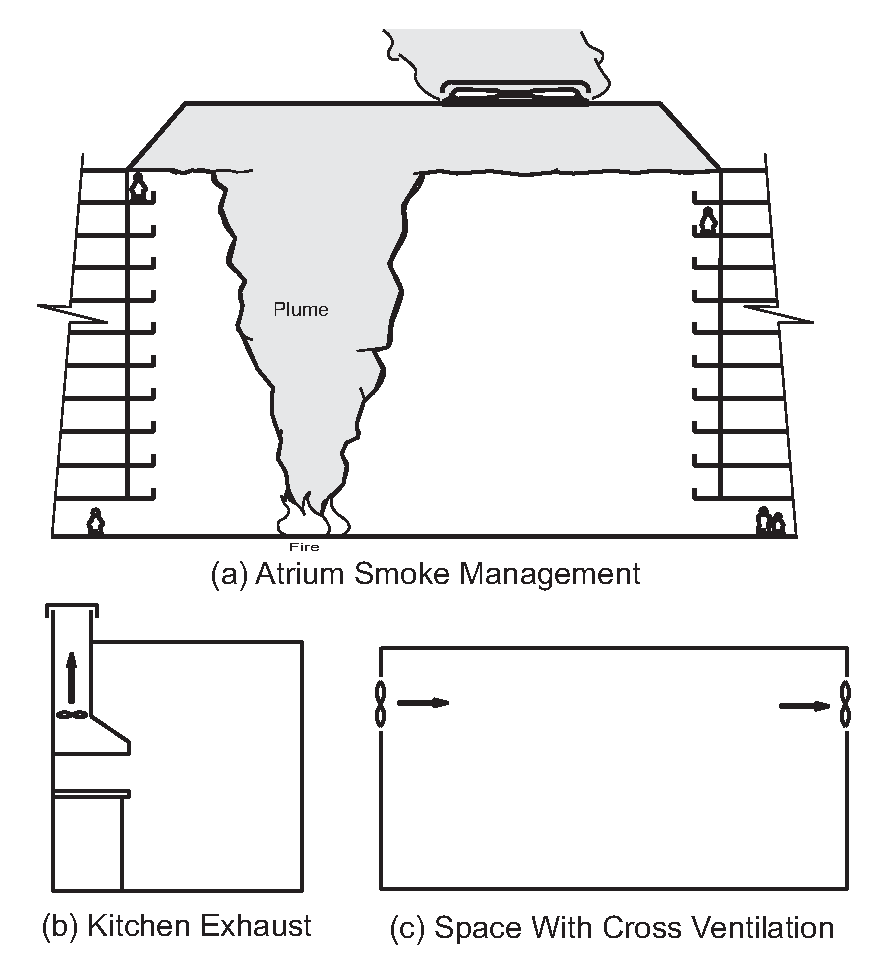
\includegraphics[width=5.0in]{FIGURES/Theory/HVAC_Fans_and_Ducts}\\
\end{center}
\caption{Some simple fan-duct systems.}
 \label{fig:Fans_and_Ducts}
\end{figure}

The flow through mechanical vents can be filtered. Filtering affects particulates such as smoke and the trace species. Filtering can be turned on at any time. Effectiveness is from 0~\% (no effect) to 100~\% which completely blocks flow of these two species.





\chapter{Heat Transfer}

This section discusses thermal radiation, convection and conduction, the three mechanisms by which heat is transferred between the gas layers and the enclosing compartment walls. Hot gases exchange heat with solid surfaces via convection and radiation. Heat is transferred through solids via conduction. Different material properties can be used for the ceiling, floor, and walls of each compartment (although all the walls of a compartment must be the same).  Additionally, each surface can be composed of up to three distinct layers.  This allows the user to deal naturally with the actual building construction.  Material thermophysical properties are assumed to be constant. Radiative transfer occurs among the fire(s), gas layers and compartment surfaces (ceiling, walls and floor).  This transfer is a function of the temperature differences and the emissivity of the gas layers as well as the compartment surfaces.  Typical surface emissivity values only vary over a small range.  For the gas layers, however, the emissivity is a function of the concentration of species which are strong radiators, predominately smoke particulates, carbon dioxide, and water.

\section{Radiation}
\label{sec:Radiation}

Radiation heat transfer is calculated between the ceiling, floor, wall layers, and fire, with the inclusion of emission and absorption by the hot gas layer~\cite{Forney_radiation}. The following assumptions are made:
\begin{itemize}
\item Each gas layer and each wall segment is assumed to be at a uniform temperature.
\item The wall segments and gas layers are assumed to be in a quasi-steady state.  In other words, the wall and gas layer temperatures are assumed to change slowly over the duration of the time step of the associated differential equation.
\item The fire is assumed to radiate uniformly in all directions giving off a fraction, $\chi_{\rm r}$, of the total heat release rate.  This radiation is assumed to originate from a single point.  Radiation feedback to the fire and radiation from the plume is not modeled in the radiation exchange algorithm.
\item The radiation emitted is assumed to be diffuse and gray.  In other words, the radiant fluxes emitted are independent of direction and wavelength. The emittance, $\epsilon$, absorptance, $\alpha$ and reflectance, $\rho$, are related via $\epsilon = \alpha = 1 - \rho$.
\item Rooms or compartments are assumed to be rectangular boxes.  Each wall is either perpendicular or parallel to every other wall.  Radiation transfer through vent openings is lost from the room.
\end{itemize}
When computing wall temperatures, CFAST partitions a compartment into four parts; the ceiling, the floor, the wall segments above the layer interface and the wall segments below the layer interface. Radiation exchange at each wall segment considers the emitted, reflected, incoming and net radiation terms.  The net radiative fluxes, $\dq_k''$, are found by solving the modified net radiation equation~\cite{SiegelandHowell:1981}:
\be
   \frac{\dq_k''}{\epsilon_k} - \displaystyle\sum_{j=1}^N \frac{1 - \epsilon_j}{\epsilon_j} \, \dq_j'' \, F_{k-j} \, \tau_{k-j} = \sigma T_k^4 - \displaystyle\sum_{j=1}^N \brackets{\sigma T_j^4 \, F_{k-j} \, \tau_{k-j}} - \frac{c_k}{A_k}
\ee
where $F_{k-j}$ is the configuration factor (fraction of radiant energy emitted by surface $k$ that is intercepted by surface $j$), $\tau_{j-k}$ is the transmittance, $\sigma$ is the Stefan-Boltzman constant, $\epsilon_k$ is the emissivity, $A_k$ is the area, and $T_k$ is the temperature of surface $k$. Reference~\cite{Forney_radiation} describes the solution of this equation.


\subsubsection{Configuration Factors}

The configuration factor, $F_{1-2}$, is the fraction of radiant energy emitted by surface 1 that is intercepted by  surface 2, and is calculated:
\be 
   F_{1-2} = \frac{1}{A_1} \int_{A_1} \int_{A_2} \frac{\cos \theta_1 \, \cos \theta_2}{\pi L^2} \, dA_2 \, dA_1 \label{eq:config_factor} 
\ee
where $L$ is the distance along the line of integration,  $\theta_1$ and $\theta_2$ are the angles for surface 1 and 2 between the respective normal vectors and the line of integration, and $A_1$ and $A_2$ are the areas of the two surfaces.  These terms are illustrated in Fig.~\ref{fig:Rad_Config_Factor}.  When the surfaces $A_1$ and $A_2$ are far apart relative to their surface area, eq (\ref{eq:config_factor}) can be approximated by assuming that $\theta_1$, $\theta_2$ and $L$ are constant over the region of integration to obtain
\begin{figure}
\begin{center}
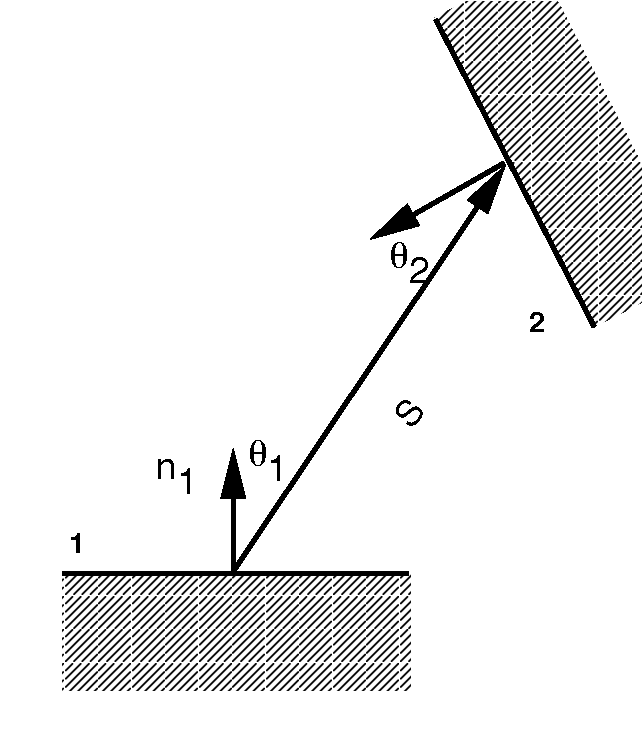
\includegraphics[width=3.0in]{FIGURES/Theory/Radiation_Config_Factor}\\
\end{center}
\caption{Setup for a configuration factor calculation between two arbitrarily oriented finite areas.}
 \label{fig:Rad_Config_Factor}
\end{figure}
\be 
   F_{1-2} = \frac{\cos \theta_1 \, \cos \theta_2}{\pi L^2} A_2 
\ee

\subsubsection{Transmittance and Absorptance} 

The transmittance of a gas volume is the fraction of radiant energy that will pass through it unimpeded and is given by
\be 
   \tau (L) = {\rm e}^{-\alpha L} 
\ee
where $\alpha$ is the absorptance of the gas volume and $L$ is a characteristic path length. The absorptance is the fraction of radiant energy absorbed by that volume. For a gray gas, $\alpha + \tau = 1$.

In general, the transmittance and absorptance are a function of wavelength.   This is an important factor to consider for the major gaseous products ($\textnormal{CO}_2$  and $\textnormal{H}_2 \textnormal{O}$); however soot has a continuous absorption spectrum which allows the transmittance and absorptance to be approximated as ``gray'' \cite{SiegelandHowell:1981} across the entire spectrum.

The gas absorptance, $\alpha_G$, is due to the combination of the $\textnormal{CO}_2$  and $\textnormal{H}_2 \textnormal{O}$ and is given by

\be \alpha_G = \alpha_{\rm H_2O} + \alpha_{\rm CO} - C\ee
where $C$ is a correction for band overlap.  For typical fire conditions, the overlap amounts to about half of the $\textnormal{CO}_2$ absorptance \cite{Tien:2002} so the gas transmittance is approximated by

\be \tau_G = 1 - \alpha_{H_2O} - 0.5 \alpha_{CO_2} \ee

The total transmittance of a gas-soot mixture is the product of the gas and soot transmittances, $\tau_T = \tau_S \tau_G$ so that

\be \tau_T = e^{-al} \brackets{1 - \alpha_{H_2O} - 0.5 \alpha_{CO_2}} \ee

In the optically thin limit the absorption coefficient, a, may be replaced by the Planck mean absorption coefficient and in the optically thick limit, it  may be replaced by the Rosseland mean absorption coefficient. For the entire range of optical thicknesses, Tien et al. \cite{Tien:2002} report that a reasonable approximation is $\alpha = k f_v T$ where $k$ is a constant that depends on the optical properties of the soot particles, $f_v$ is the soot volume fraction and $T$ is the soot temperature in Kelvin. Values of $a$, have been found to be about constant for a wide range of fuels \cite{Tien:1978}.   The soot volume fraction, $f_v$, is calculated from the soot mass, soot density and layer volume.  The soot is assumed to be in thermal equilibrium with the gas layer.

Edwards' absorptance data for $\textnormal{H}_2 \textnormal{O}$ and $\textnormal{CO}_2$ are reported \cite{Edwards:1985} as log(emissivity) versus log(pressure-pathlength), with  log(gas concentration) as a parameter. For each gas, these data were incorporated into a look-up table, implemented as a two-dimensional array of log(emissivity) values, with indices based on temperature and gas concentration.  It is assumed that absorptance and emittance are equivalent for the gaseous species as well as for soot.

An effective path length ( mean beam length, L) treats an emitting volume as if it were a hemisphere of a radius such that the flux impinging on the center of the circular base is equal to the average boundary flux produced by the real volume. The value of this radius is approximated as \cite{Tien:1978, Hottel:1942} $L = c 4 V / A$ where $L$ is the mean beam length in meters, $c$ is a constant (approximately 0.9, for typical geometries), $V$ is the emitting gas volume m$^3$ and $A$ is the surface area (m$^2$) of the gas volume. The volume and surface area are calculated from the dimensions of the layer.

For each gas, the log(absorptance) is estimated from the look-up table for that gas  by  interpolating both the log(temperature) and log(concentration) domains. In the event that the required absorptance lies outside the temperature or concentration range of the look-up table, the nearest acceptable value is returned. Error flags are also returned, indicating whether each parameter was in or out of range and, in the latter case, whether it was high or low.  This entire process is carried out for both $\textnormal{CO}_2$  and $\textnormal{H}_2 \textnormal{O}$.

\section{Convection}

\subsection{Walls, Ceilings, and Floors}

In general, convective heat flux to a solid surface is given by:
\be
   \dqc'' = h \, \brackets{\Tg - \Ts}  \label{convective_heat_flux}
\ee
The convective heat transfer coefficient, $h$, is a function of the gas properties, temperature, and velocity. In CFAST, simple correlations for natural convection are used since the gas velocity is unknown:
\be
   h = C {|\Tg - \Ts|}^{1/3}
\ee
where $C$ is an empirical coefficient (1.52 for the horizontal floors and ceilings and 1.31 for the vertical walls~\cite{Holman:1990}), $\Tg$ is the gas temperature adjacent to the surface, and $\Ts$ is the surface temperature.

\subsection{Ceiling Jet}

Relatively early in the development of a fire, fire-driven ceiling jets and gas-to-ceiling convective heat transfer can play a significant role in room-to-room smoke spread and in the response of near-ceiling mounted detection hardware.  Cooper \cite{Cooper:1991} details a model and computer algorithm to predict the instantaneous rate of convective heat transfer from fire plume gases to the overhead ceiling surface in a room of fire origin.  The room is assumed to be a rectangular parallelepiped and, at times of interest, ceiling temperatures are simulated as being uniform.  Also presented is an estimate of the convective heat transfer due to ceiling-jet driven wall flows.  The effect on the heat transfer of the location of the fire within the room is taken into account.  This algorithm has been incorporated into the CFAST model.  In this section, we provide an overview of the model.  Complete details are available in reference [\cite{Cooper:1991}.

A schematic of a fire, fire plume, and ceiling jet is shown in Fig.~\ref{fig:CeilJet}. The buoyant fire plume rises from the height $Z_{fire}$ toward the ceiling.  When the fire is below the layer interface, its mass and enthalpy flow are assumed to be deposited into the upper layer at height $Z_{layer}$.  Having penetrated the interface, a portion of the plume typically continues to rise toward the ceiling.  As it impinges on the ceiling surface, the plume gases turn and form a relatively high temperature, high velocity, turbulent ceiling jet which flows radially outward along the ceiling and transfers heat to the relatively cool ceiling surface.  The convective heat transfer rate is a strong function of the radial distance from the point of impingement, reducing rapidly with increasing radius.  Eventually, the relatively high temperature ceiling jet is blocked by the relatively cool wall surfaces \cite{Cooper:1990a}.  The ceiling jet then turns downward and outward in a complicated flow along the vertical wall surfaces \cite{Cooper:1988, Jaluria:1989} .  The descent of the wall flows and the heat transfer from them are eventually stopped by upward buoyant forces.  They are then buoyed back upward and mix with the upper layer.

\begin{figure}
\begin{center}
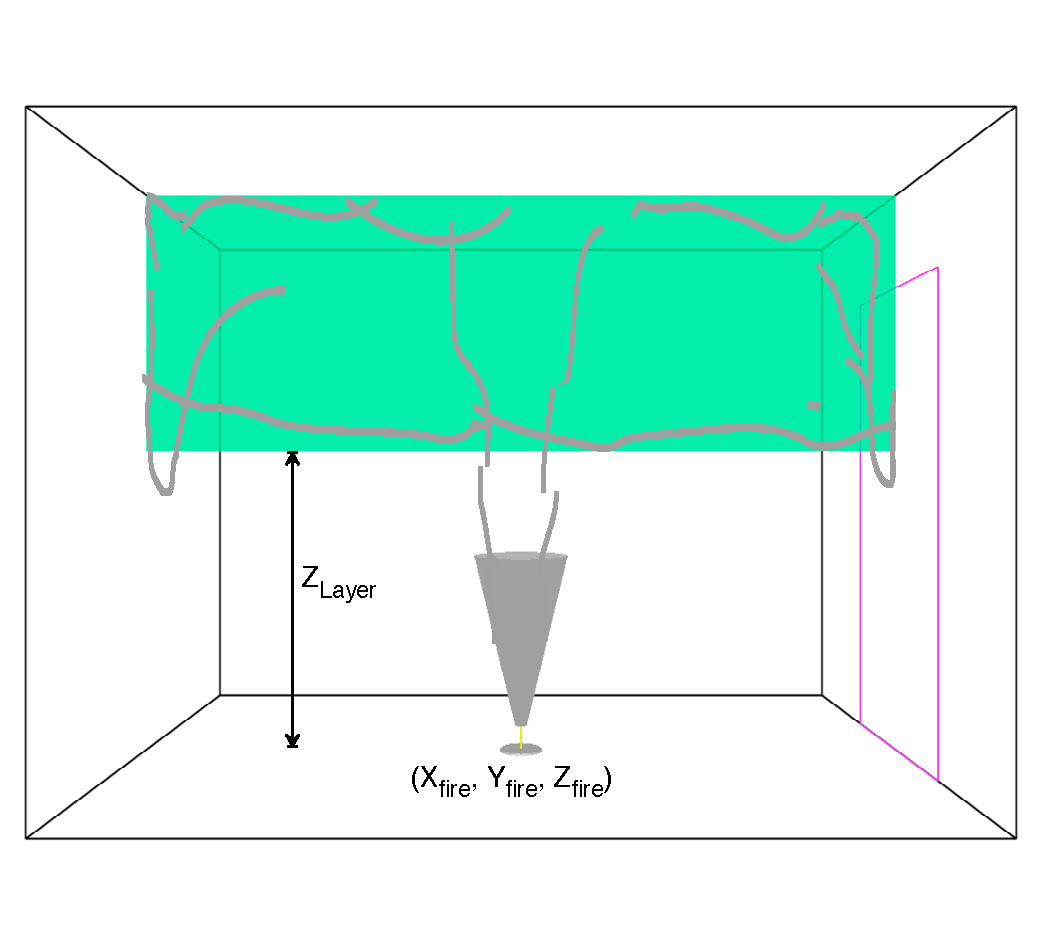
\includegraphics[width=4.0in]{FIGURES/Theory/CeilJet}\\
\end{center}
\caption{Convective heat transfer to ceiling and wall surfaces via the ceiling jet.}
 \label{fig:CeilJet}
\end{figure}

The average convective heat transfer from the ceiling jet gases to the ceiling surface, $Q_{ceil}$, can be expressed in integral form as

\be Q_{ceil} = \int_0^{X_{wall}} \int_0^{Y_{wall}} q_{ceil}\dprime (x,y) dx dy \ee

The instantaneous convective heat flux, $q_{ceil}\dprime (x,y)$ can be determined as derived by Cooper \cite{Cooper:1991} as

\be q_{ceil}\dprime (x,y) = h \brackets{T_{ad} - T_{ceil}} \ee
where $T_{ad}$ is a characteristic ceiling jet temperature that would be measured adjacent to an adiabatic lower ceiling surface, and $h$ is a heat transfer coefficient.  $h$ and $T_{ad}$ are given by

\be \frac{h}{\tilde{h}} =
\left\{
\begin{array}{cc}
8.82 Re_H^{-1/2} Pr^{-2/3} \brackets{1 - \brackets{5 - 0.284 Re_H^{2/5}}\rH} & 0 \le \rH < 0.2 \\
\\
0.283 Re_H^{0.3} Pr^{-2/3} \brackets{\rH}^{-1.2} \frac{\rH - 0.0771}{\rH + 0.279} & 0.2 \le \rH
\end{array}
\right.
\ee

\be \frac{T_{ad} - T_u}{T_u {Q_H^*}^{2/3}} =
\left\{
\begin{array}{cc}
10.22 - 14.9 \rH & 0 \le \rH < 0.2 \\
\\
8.39 f\brackets{\rH} & 0.2 \le \rH
\end{array}
\right.
\ee
where

\be f\brackets{\rH} = \frac{1 - 1.10 \brackets{\rH}^{0.8}+ 0.808  \brackets{\rH}^{1.6}}
{1 - 1.10 \brackets{\rH}^{0.8}+ 2.20  \brackets{\rH}^{1.6} + 0.690 \brackets{\rH}^{2.4}}
\ee

\be r = \sqrt{\brackets{X-X_{fire}}^2 + \brackets{Y-Y_{fire}}^2} \ee
\be \tilde{h} = \rho_u c_p g^{1/2} H^{1/2} {Q_H^*}^{1/3} \; , \;
Re_H = \frac{g^{1/2} H^{3/2} {Q_H^*}^{1/3}}{\nu_u}  \; , \;
Q_H^* = \frac{Q}{\rho_u c_p T_u g^{1/2} H^{5/2} } \ee

\be Q =
\left\{
\begin{array}{cc}
Q_{f,C} \brackets{\frac{\sigma \dot{M}^*}{1 + \sigma}}& Z_{fire} < Z_{layer} < Z_{ceil} \\
\\
Q_{f,C} & {\begin{array}{c}
Z_{fire} \ge Z_{layer} \\
Z_{layer} = Z_{ceil}
\end{array} }
\end{array}
\right.
\; , \;
 \dot{M}^* =
\left\{
\begin{array}{cc}
0 & -1 < \sigma \le 0 < 0.2 \\
\\
\frac{1.04599 \sigma + 0.360391 \sigma^2}{1 + 1.37748 \sigma + 0.360391 \sigma^2} & \sigma > 0
\end{array}
\right.
\ee

\be \sigma = \frac{1 - \frac{T_u}{T_l}+C_T {Q_{EQ}^*}^{2/3}}{\frac{T_u}{t_l}}
\; , \;
C_T = 9.115
\; , \;
Q_{EQ}^* = \brackets{\frac{0.21 Q_{fc}}{c_p T_l \dot{m}_p}} \ee

In the above, $H$ is the distance from the (presumed) point source fire and the ceiling, $X_{fire}$  and $Y_{fire}$ are the position of the fire in the room, $Pr$ is the Prandtl number (taken to be 0.7) and $\nu$ is the kinematic viscosity of the upper layer gas which is assumed to have the properties of air and can
be estimated from $\nu = 0.04128 x 10^7 T_u^{5/2} /\brackets{T_u + 110.4}$. $Q_H^*$ and $Q_{EQ}^*$ are dimensionless numbers and are measures of the strength of the plume at the ceiling and the layer interface, respectively.

When the ceiling jet is blocked by the wall surfaces, the rate of heat transfer to the surface increases.  Reference \cite{Cooper:1991} provides details of the calculation of wall surface area and convective heat flux for the wall surfaces.

 \section{Conduction}

The heat conduction equation is solved in the direction normal to the solid surface using non-uniformly spaced nodes and a second order accurate central difference scheme for the spatial derivatives and a semi-implicit time marching scheme. At each time step, the internal temperatures are updated in time until net the net convective and radiative heat flux striking the wall is consistent with the heat flux into the surface~\cite{Moss:1992}
\be
   \dq'' = -k \, \frac{dT}{dx} \Big|_{x=0}
\ee
where $k$ is the thermal conductivity of the solid.  This solution strategy requires a differential algebraic equation (DAE) solver that can simultaneously solve both differential and algebraic equations.  With this method, only one or two extra equations are required per wall segment (two if both the interior and exterior wall segment surface temperatures are computed).  This solution strategy is more efficient than the method of lines since fewer equations need to be solved. Conduction is then coupled to the gas phase energy exchange.

A non-uniform array of internal nodes is used to capture steep gradients in temperature near the surace. Define a penetration depth of
\be
   x_p = 2 \sqrt{\alpha \, t_{\rm end}} \; \hbox{erfc}^{-1} \brackets{0.05}
\ee
where $\hbox{erfc}^{-1}$ denotes the inverse of the complementary error function. The value $x_p$ is the location in a semi-infinite wall where the temperature rise is 5~\% after $t_{\rm end}$ seconds. Eighty percent of the nodes are placed on the interior side of $x_p$ and the remaining 20~\% are placed on the exterior side.

To illustrate the method, consider a one room case with one active wall.  There are four gas equations (pressure, upper layer volume, upper layer temperature, and lower layer temperature) and one wall temperature equation.  Implementation of the gradient matching method requires that storage be allocated for the temperature profile at the previous time, t, and at the next time, $t + \Delta t$.  Given the profile at time t and values for the five unknowns at time $t + \Delta t$ (initial guess by the solver), the temperature profile is advanced from time t to time $t + \Delta t$.  The temperature gradient at $x = 0$ is computed followed by the residuals for the five equations.  The DAE solver adjusts the solution variables and the time step until the residuals for all the equations are below an error tolerance.  Once the solver has completed the step, the array storing the temperature profile for the previous time is updated, and the DAE solver is ready to take its next step.

Heat transfer between connected compartments is modeled by merging the back surfaces of the connected ceiling and floor of the compartments or the back wall surfaces of the connected horizontal compartments.  A heat conduction problem is solved for the merged walls using a temperature boundary condition for both the near and far wall.  As before, temperatures are determined by the DAE solver so that the heat flux striking the wall surface (both interior and exterior) is consistent with the temperature gradient at that surface.

For horizontal heat transfer between compartments, the connections may be between partial wall surfaces, expressed as a fraction of the wall surface. CFAST first estimates conduction fractions analogous to radiative configuration factors.    For example, if only one half of the rear wall in one compartment is adjacent to the front wall in a second compartment, the conduction fraction between the two compartments is 1/2.   Once these fractions are determined, an average flux, $\dq_{\rm avg}''$, is calculated using
\be
   \dq_{\rm avg}'' = \sum_{\rm walls} \, F_{ij} \dq_j''
\ee
where $F_{ij}$ is the fraction of flux from wall $i$ that contributes to wall $j$, $\dq_j''$ is the flux striking wall $j$.

\section{Computing Target Heat Flux and Temperature}

The calculation of the radiative heat flux to a target is similar to the radiative heat transfer calculation discussed previously.  The main difference is that CFAST does not compute feedback from the target to the wall surfaces or gas layers.  The target is simply a probe or sensor that does not interact with the modeled environment. There are four components of heat flux to a target: fires, walls (including the ceiling and floor), gas layer radiation and gas layer convection.

\subsubsection{Heat Flux from a Fire to a Target}

Assuming the fire to be a point source of radiant energy, the heat flux to a target at a distance $R$ whose surface normal forms an angle $\theta$ with the line connecting the fire and target is given by:
\be
   \dqr'' = \frac{\chi_{\rm r} \, \dQ}{4 \pi \, R^2} \, \cos \brackets{\theta} \, \tau_{\rm u} \, \tau_{\rm l}
\ee
where the $\tau_{\rm u}$ and $\tau_{\rm l}$ are the transmissivity of the upper and lower layer, respectively.

\subsubsection{Radiative Heat Flux from a Wall Segment to a Target}

Figure \ref{fig:Rad_Gases} illustrates terms used to compute heat flux from a wall segment to a target. The flux, $q\dprime_{w,t}$, from a wall segment to a target can then be computed using
\be
   \dqr'' = \frac{A_{\rm w} \dq_{\rm w,out}'' \, F_{\rm w-t}}{A_{\rm t}} \, \tau_{\rm u} \, \tau_{\rm l} \label{eq:wall_target_flux} \ee
where $\dq_{\rm w,out}''$  is the flux leaving the wall segment, $A_{\rm w}$, $A_{\rm t}$ are the areas of the wall segment and target respectively, $F_{\rm w-t}$  is the configuration factor, and $\tau_{\rm u}$ and $\tau_{\rm l}$ are the transmissivity of the upper and lower layer, respectively.
\begin{figure}
\begin{center}
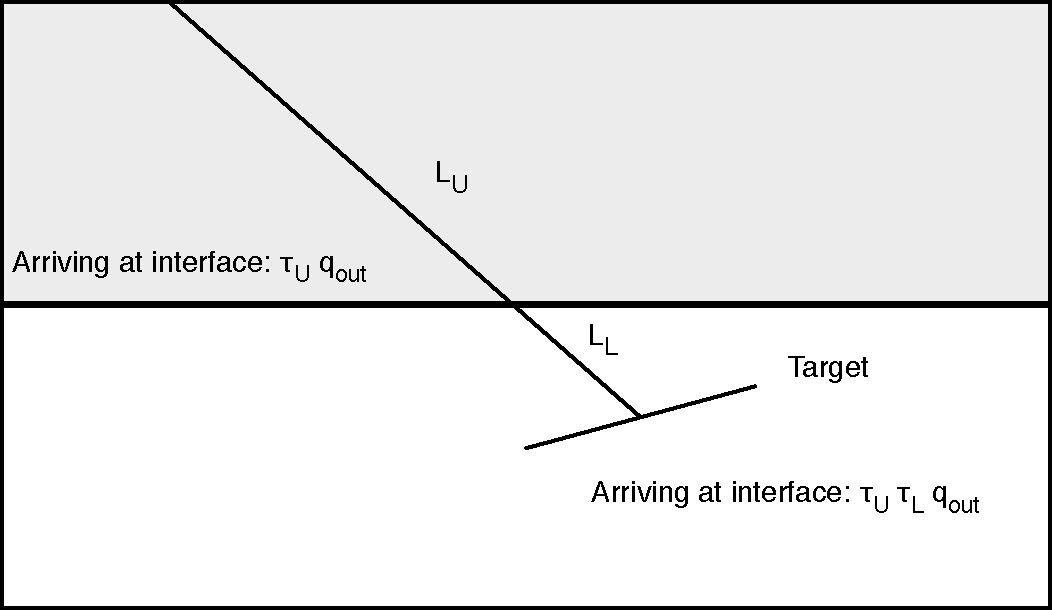
\includegraphics[width=5.0in]{FIGURES/Theory/Radiation_Gases}\\
\end{center}
\caption{Radiative heat transfer from the upper and lower layer gas to a target in the lower layer.}
 \label{fig:Rad_Gases}
\end{figure}

\subsubsection{Radiation from the Gas Layer to the Target}

Figure \ref{fig:Rad_Gases} illustrates the setup for calculating the heat flux from the gas layers to the target.  The upper and lower gas layers in a room contribute to the heat flux striking the target if the layer absorptance is non-zero. Let $q_{w,t,gas}\dprime$ denote the flux striking the target due to the gas g in the direction of wall segment w. Then

\be q_{w,t,gas}\dprime =
\left\{
\begin{array}{ll}
\sigma F_{t-w} \brackets{T_L^4 \alpha_L \tau_U + T_U^4 \alpha_U} & w \textnormal{ is in the lower layer}\\
\sigma F_{t-w} \brackets{T_U^4 \alpha_U \tau_L + T_L^4 \alpha_L} & w \textnormal{ is in the upper layer}
\end{array}
\right. \label{eq:Rad_Gases} \ee

The total target flux due to the gas (upper or lower layer) is obtained by summing eq (\ref{eq:Rad_Gases} over each wall segment or

\be q_{g,t}\dprime = \sum_w = q_{w,t,gas}\dprime  \ee

{\bf Computing the Steady State Target Temperature:} The steady state target temperature, $T_t$ can be found by solving an energy balance on the target; namely

\be \epsilon_t \sigma T_t^4 = \epsilon_t q_{r,in} + h \brackets{T_g - T_t} \label{eq:Target_Temp} \ee
Note that the local gas temperature, $T_g$, in the convection calculation, $h \brackets{T_g - T_t}$, is taken to be either the upper layer temperature if the target is located in the upper layer, the lower layer temperature if the target is located in the lower layer, or the plume centerline temperature if the target is located directly above a fire source.

Let $f(T_t)$ be the difference between the left and right hand side of equation (\ref{eq:Target_Temp}).  Then this equation may be solved using the Newton iteration

\be T_{new} = T_{old} - \frac{f(T_{old})}{f^\prime(T_{old})} \label{eq:Target_Newton} \ee

Equation (\ref{eq:Target_Newton}) is iterated until the difference $T_{new} - T_{old}$ is sufficiently small.

{\bf Computing the Transient Rectangular Target Temperature:}
A transient target temperature may be computed using two different methods
depending on whether the target is assumed to be thin or thick.  A thin target
is presumed to have a constant interior temperature profile. A differential equation model may then be used to estimate the
temperature rise (or fall) based upon the thermal properties of the target and the
heat flux striking the front and back sides; namely

\be c \rho V \frac{dT}{dt} = A(q''_f+q''_b) \label{eq:Target_ODE} \ee

where $c$, $\rho$ and $V$ are the the specific heat, density and volume of the target, $A$ is the cross-sectional area of the target and the two $q''$ terms are the heat flux (due to all sources) striking the front and back sides of the target.

Equation (\ref{eq:Target_ODE}) may be solved implicitly or explicitly.  When solved implicitly, the target temperature is added to the set of solution variables and equation (\ref{eq:Target_ODE}) is added to the equation set solved by DASSL.
When solved explicitly, equation (\ref{eq:Target_ODE}) is solved as a stand-alone equation advancing the target temperature in time.


If the target is thick then it is presumed that the temperature profile within the target varies as a function of depth and therefore a partial differential equation model must be used to estimate the changing profile; namely the heat equation

\be \frac{\partial T}{\partial t} = \frac{k}{\rho C}\frac{\partial^2T}{\partial x^2}
\label{eq:Target_PDE} \ee
where $k$, $\rho$ and $C$ are the thermal conductivity, density and heat capasity of the target.  As with the standard heat conduction model discussed later, the target heat conduction model in CFAST couples the solid to the gas phase using the relation

\be q''=-k\frac{dT}{dx} \label{eq:Target_Fourier}\ee

where $q''$ is the heat flux striking the target (again due to all sources).  This equation is the statment that the flux striking the target must be consistent with the temperature gradient at the surface.

Equation (\ref{eq:Target_PDE}) may be solved implicitly or explicitly.  When solved implicitly, the target temperature is added to the set of solution variables and equation (\ref{eq:Target_Fourier}) (not equation (\ref{eq:Target_PDE}) is added to the equation set solved by DASSL.
When solved explicitly, equation (\ref{eq:Target_PDE}) is solved as a stand-alone equation advancing the temperature profile in time.

{\bf Computing Transient Cable Target Heat Transfer:}

\newcommand{\Dt}{\Delta t}
\newcommand{\Dr}{\Delta r}
\newcommand{\Tipo}{T_{i+1}^{n+1}}
\newcommand{\Ti}{T_{i}^{n+1}}
\newcommand{\Timo}{T_{i-1}^{n+1}}

This section describes a CFAST implementation of a model for
predicting electrical cable failure first proposed
by Andersson and Van Hees Ref.~\cite{Andersson:2005}
and later implemented by McGrattan
in FDS~\cite{CAROLFIRE} .  This model uses a simple one-dimensional heat
transfer calculation, under the assumption that the cable can
be treated as a homogenous cylinder~\cite{Andersson:2005}.

The heat flux used to generate the heat transfer in the cable is provided
by CFAST which models the thermal environment of the compartment where
the cable is located.  In most realistic fire  scenarios, the heat flux
to the cable is not axially-symmetric.  CFAST therefore uses the maximum
heat flux value when modeling cable failure.

1D heat transfer may be computed within a cylindrically symmetric target
by splitting it into $N$ concentric control volumes and performing
an energy balance on each.  The energy balance for the $i$'th control
volume for $i=1\cdots N-1$, is

\begin{equation}
c\rho V_i\Delta T_i=(\dot{q}_i-\dot{q}_{i-1})\Dt
\label{eq:cylheat1}
\end{equation}

\noindent where $c\rho V_i\Delta T_i$ represents the change in internal
energy
and $(\dot{q}_i-\dot{q}_{i-1})\Dt$ represents the net heat flow across the
control volume's inner and outer boundary surface over a $\Dt$ time period.
The energy balance for the outermost or $N$'th control volume is similar
\begin{equation}
c\rho V_N\Delta T_N=(\dot{q}_{ext}''A_N-\dot{q}_{N-1})\Dt
\label{eq:cylheat2}
\end{equation}
with $\dot{q}_{ext}''A_N$ used to specify a boundary condition,
the combined net radiative and convective heat flux incident
on the the cylindrical target's outer surface.

\begin{figure}[h]
\begin{center}
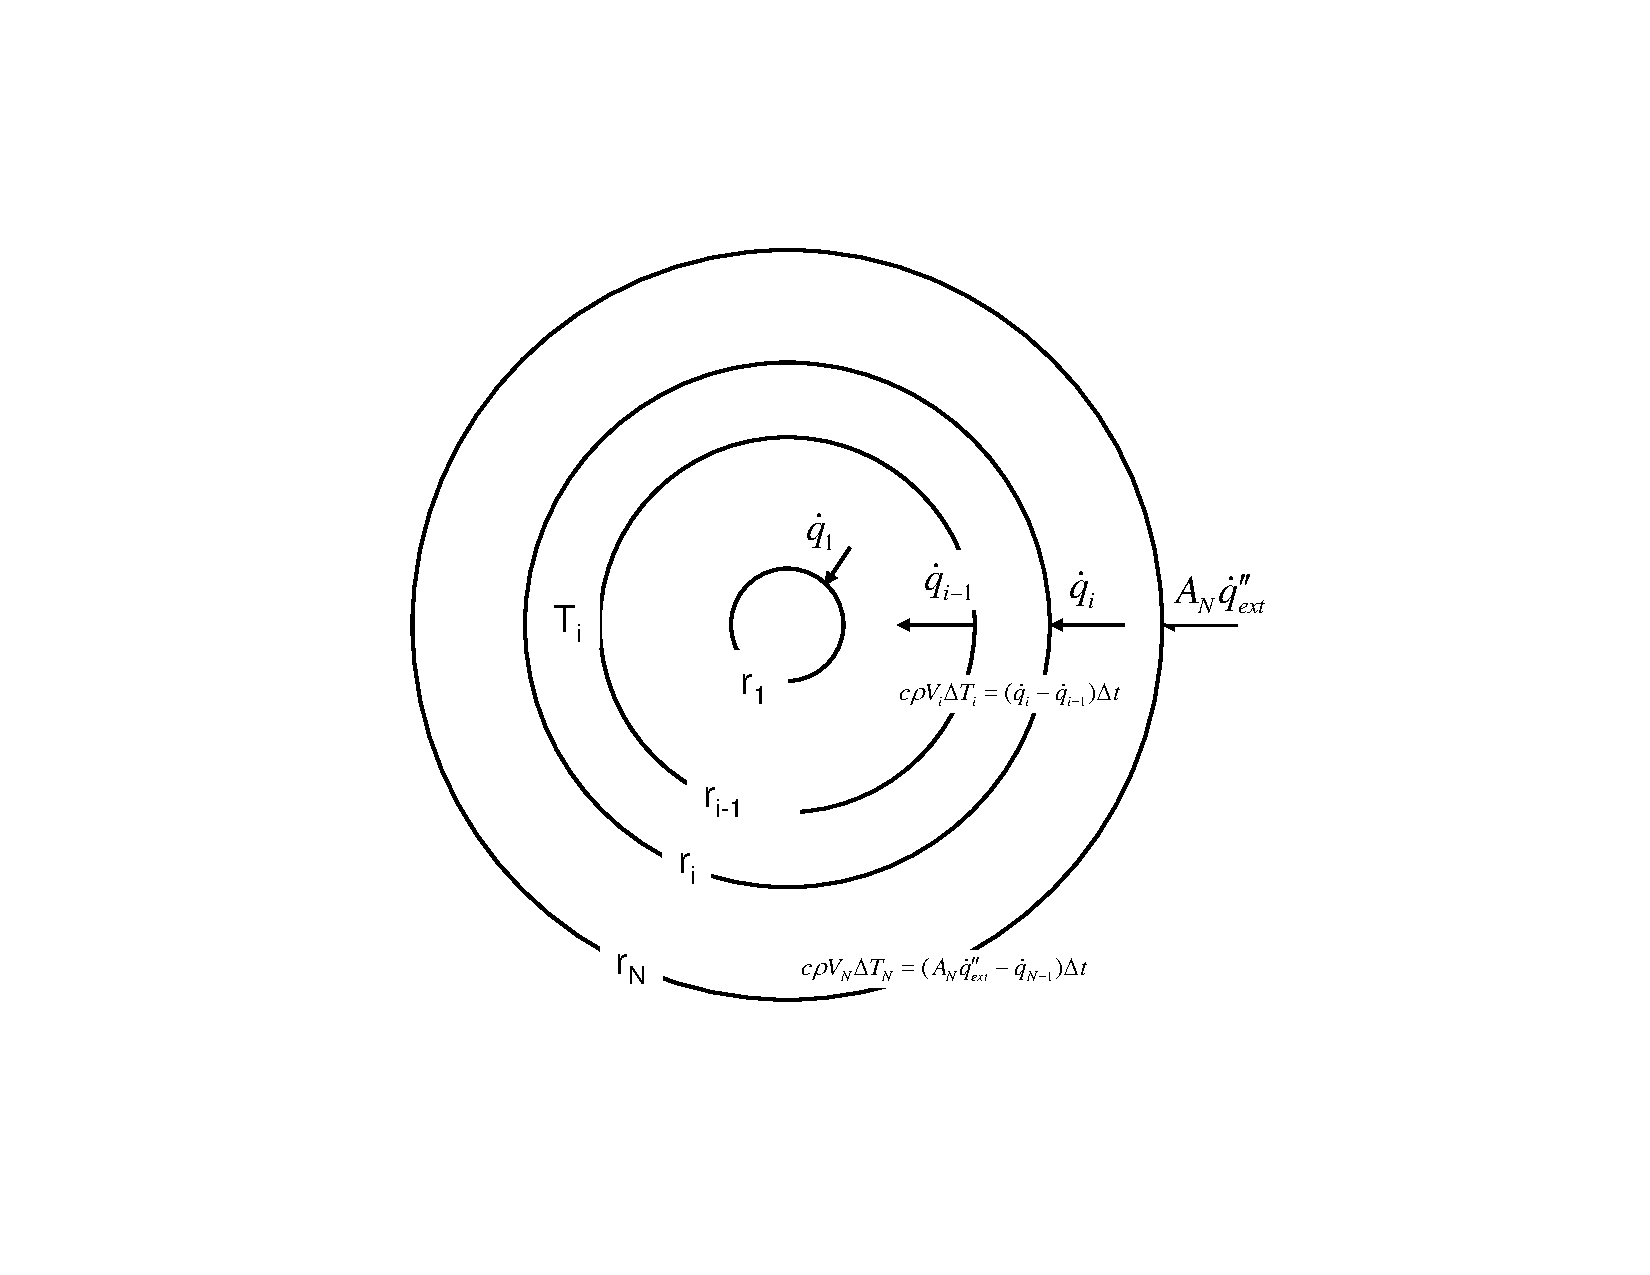
\includegraphics[width=5.0in]{FIGURES/Theory/cylheat}\\
\end{center}
\caption{Schematic of a control volume for heat transfer in a cylindrical object.}
 \label{fig:cylheat}
\end{figure}
As illustrated in Figure \ref{fig:cylheat}, the $i$'th control volume has
volume $V_i$, temperature $T_i$ and heat flow at the inner
and outer boundaries of $\dot{q}_{i-1}$ and $\dot{q}_i$ respectively.
The $i$'th control volume has length $L$ and inner and outer radius
$r_{i-1}$ and $r_i$ where $r_i=i\Dr$ and $\Dr=R/N$.
The density and specific heat of material in all control volumes is
$c$ and $\rho$.

The right hand sides of equations \ref{eq:cylheat1} and (\ref{eq:cylheat2}) may be expressed in terms of temperature using
Fourier's law and noting that $\dot{q}_i=\dot{q}''_iA_i$ to obtain
\begin{equation}
c\rho V_i\Delta T_i=(\dot{q}''_iA_i-\dot{q}''_{i-1}A_{i-1})\Dt
=
\left[
k\left(\frac{T_{i+1}-T_i}{\Dr}\right)A_i-k\left(\frac{T_{i}-T_{i-1}}{\Dr}\right)A_{i-1}
\right]
\label{eq:cylheat2a}
\end{equation}

\noindent The volume of the $i$'th control volume is given by
\begin{eqnarray*}
V_i&=&\pi(r_i^2-r_{i-1}^2)L
=\pi\Dr(r_i+r_{i-1})L
=2\pi\Dr(i-0.5) L
\label{eq:cylheat3}
\end{eqnarray*}

\noindent The area, $A_i$, of the outer boundary surface of the $i$'th
control volume is given by
\begin{eqnarray*}
A_i=2\pi r_iL
=2\pi \Dr iL
\label{eq:cylheat4}
\end{eqnarray*}

\noindent Using the ratio $A_i/V_i=i/(\Dr(i-0.5))$
and $\Delta T_i=\Ti-T_i^n$,
equation (\ref{eq:cylheat2a}) may be simplified to
\begin{eqnarray}
\Ti-T_i^n&=&\frac{\Dt}{\rho c}
\left[
\left(\frac{\Tipo-\Ti}{\Dr}\right)
\frac{A_i}{V_i}-
\left(\frac{\Ti-\Timo}{\Dr}\right)
\left(\frac{A_{i-1}}{V_i}\right)
\right]
\nonumber\\
&=&\frac{\Dt}{\Dr^2}\frac{k}{\rho c}
\left[
\left(\Tipo-\Ti\right)
\left(\frac{i}{i-0.5}\right)-
\left(\Ti-\Timo\right)
\left(\frac{i-1}{i-0.5}\right)
\right]\nonumber\\
&=&\frac{\alpha\Dt}{\Dr^2(i-0.5)}
\left[
\left(\Tipo-\Ti\right)
i-
\left(\Ti-\Timo\right)
(i-1)
\right]
\label{eq:cylheat6}
\end{eqnarray}

\noindent where $\alpha-k/(\rho c)$.  Defining $C_i$ and $D_i$ as
\begin{eqnarray*}
C_i&=&\frac{\alpha\Dt}{\Dr^2}\left(\frac{i-1}{i-0.5}\right)\\
D_i&=&\frac{\alpha\Dt}{\Dr^2}\left(\frac{i}{i-0.5}\right),\\
\end{eqnarray*}
\noindent noting that $C_i+D_i=2\frac{\alpha\Dt}{\Dr^2}$
for $i=1\cdots N-1$ and
substituting into (\ref{eq:cylheat6}) results in

\begin{equation}
-C_i\Timo+(1+2\frac{\alpha\Dt}{\Dr^2})\Ti-D_i\Tipo=T_i^n
\label{eq:cylheat8}
\end{equation}

\noindent The energy balance for the $N$'th (outermost) control volume may be obtained by substituting $\Dr q''_{ext}/k$ for $\Tipo-\Ti$ in equation (\ref{eq:cylheat6}) to obtain
\begin{eqnarray*}
T_N^{n+1}-T_N^n=\frac{\alpha\Dt}{\Dr^2(N-0.5)}
\left[\frac{\Dr\dot{q}''_{ext}}{k}N-(T_N^{n+1}-T_{N-1}^{n+1})(N-1)\right]
\end{eqnarray*}

\noindent then substituting $C_N$ and $D_N$ and simplifying
to obtain

\begin{equation}
-C_NT_{N-1}^{n+1}+(1+C_N)T_N^{n+1}=T_N^n+D_N\frac{\Dr}{k}q''_{ext}
\label{eq:cylheat10}
\end{equation}

Equations (\ref{eq:cylheat8}) and (\ref{eq:cylheat10}) represent a  tri-diagonal linear system of equations which when written in matrix form
are given by
\begin{equation}
\left(
\begin{array}{ccccccccc}
  1+D_1 & -D_1 &  &  &  &  &  &  &  \\
   &  &  &  &  &  &  &  &  \\
   &  &\ddots  &  &  &  &  &  &  \\
   &  &  &  &  &  &  &  &  \\
   &  &  & -C_i &1+2\frac{\alpha\Dt}{\Dr^2}  &D_i  &  &  &  \\
   &  &  &  &  &  &  &  &  \\
   &  &  &  &  & \ddots &  &  &  \\
   &  &  &  &  &  &  &  &  \\
   &  &  &  &  &  &-C_N  &1+C_N  &
\end{array}
\right)
\left(
  \begin{array}{c}
    T_1^{n+1}\\
    T_2^{n+1}\\
    \vdots\\
    T_{i-1}^{n+1} \\
    T_i^{n+1} \\
    T_{i+1}^{n+1}\\
    \vdots\\
    T_{N-1}^{n+1}\\
    T_N^{n+1}
  \end{array}
\right)
=
\left(
  \begin{array}{c}
    T_1^{n}\\
    T_2^{n}\\
    \vdots\\
    T_{i-1}^{n} \\
    T_i^{n} \\
    T_{i+1}^{n}\\
    \vdots\\
    T_{N-1}^{n}\\
    T_N^{n}+D_N\frac{\Dr}{k}\dot{q}''_{ext}
  \end{array}
\right)
\label{eq:matrix}
\end{equation}

\noindent Equation (\ref{eq:matrix}) is then used to
advance the cable's temperature profile by $\Delta t$.






\chapter{Fire Protection Devices}



\section{Sprinkler and Heat Detector Activation}

The link temperature of a sprinkler or heat detector is modeled using the differential equation~\cite{Heskestad:1976}:
\be
   \frac{d \TL}{dt} = \frac{\sqrt{v}}{\rm RTI} \brackets{\Tg - \TL}  \label{eq:RTI}
\ee
where $\TL$ and $\Tg$ are the link and gas temperatures, $v$ is the ceiling jet velocity, and RTI (Response Time Index) is a measure of the sensor's thermal inertia. The gas temperature and velocity obtained from the ceiling jet algorithm, Section~\ref{Ceiling_Jet_Algorithm}. Rooms without fires do not have ceiling jets, in which case the upper layer temperature is used, along with a fixed velocity of 0.12~m/s. The link and gas temperatures and the velocity are functions of time; the RTI is a constant for a given detector type. The detector equation is solved numerically using the semi-implicit updating scheme:
\be
   \frac{\TL^{n+1}-\TL^n}{\delta t} = \frac{1}{2} \left( \frac{\sqrt{v^n}}{\rm RTI} \brackets{\Tg^n - \TL^n}  + \frac{\sqrt{v^{n+1}}}{\rm RTI} \brackets{\Tg^{n+1} - \TL^{n+1}}  \right) \label{eq:RTI_rewritten}
\ee
where the superscript $n$ denotes the value at the current time, and $\delta t$ is the time step.


\section{Fire Suppression} \label{sec:suppression}

Fire suppression by water is predicted using a simple empirical model developed by Madrzykowski \cite{Madrzykowski:1992} and Evans~\cite{Evans:1993}. After activation of the sprinkler, $t > t_{\rm act}$, the heat release rate is assumed to decrease exponentially:
\be
   \dQ(t) = \dQ(t_{\rm act}) \; {\rm e}^{-(t-t_{\rm act}) /\tau}   \quad ; \quad \tau = 3 u_{\rm w}^{-1.8}
\ee
where $u_{\rm w}$ is the water spray density, expressed in units of m/s. The product species mass production rates are reduced by the same amount as the heat release rate.

There are assumptions and limitations in this approach. Its main deficiency is that it assumes that sufficient water is applied to the fire to cause a decrease in the rate of heat release. This suppression model cannot handle the case when the fire overwhelms the sprinkler.  The suppression model as implemented does not include the effect of a second sprinkler. Detection of all sprinklers are noted but their activation does not make the fire go out any faster. Further, multiple fires in a room imply multiple ceiling jets. It is not clear how the two ceiling jets should interact. When there is more than one fire, the detection algorithm uses the fire that results in the highest ceiling jet temperature in order to calculate the sprinkler link temperature.

\section{Species Concentration and Deposition}

CFAST uses a combustion chemistry scheme based on a carbon-hydrogen-oxygen balance.  The scheme is applied in three places.  The first is burning in the portion of the plume which is in the lower layer of the compartment of fire origin.  The second is the portion in the upper layer, also in the compartment of origin.  The third is in the vent flow which entrains air from a lower layer into an upper layer in an adjacent compartment.  Included in the combustion calculation is the generation and transport of a number of species that may be produced by a fire.  These species include unburned fuel, nitrogen, oxygen, carbon monoxide, carbon dioxide, hydrogen, carbon (assumed to be soot produced by the fire), hydrogen cyanide, hydrogen chloride, and an arbitrary trace species.

\subsection{Species Transport}

The species transport in CFAST is primarily a matter of bookkeeping to track individual species mass as it is generated by a fire, transported through vents, or mixed between layers in a compartment.  When the layers are initialized at the start of the simulation, they are set to ambient conditions.  These are the initial temperature prescribed by the user, and 23 \% by mass fraction (21 \% by volume fraction) oxygen, 77 \% by mass fraction (79 \% by volume fraction) nitrogen, a mass concentration of water prescribed by the user as a relative humidity, and a zero concentration of all other species.  As fuel is burned, the various species are produced in direct relation to the mass of fuel burned (this relation is the species yields prescribed by the user for the fuel burning).  Since oxygen is consumed rather than produced by the burning, the `yield' of oxygen is negative, and is set internally to correspond to the amount of oxygen used to burn the fuel (within the constraint of available oxygen limits discussed in sec. \ref{sec:Oxygen_Limit}). Two special separate species calculations are included in the model, a time-integrated value for a generic toxic species, Ct, and an arbitrary trace species, TS.  Both are assumed not to be part of the overall mass balance, but are rather generated by a fire and transported through a structure in a manner identical to other species.

Each unit mass of a species produced by a fire is carried in the flow to the various rooms and accumulates in the layers.  The model keeps track of the mass of each species in each layer, and knows the volume of each layer as a function of time.  The mass divided by the volume is the mass concentration, which along with the relative molecular mass gives the concentration in volume percent or parts per million as appropriate. Filters can be used in mechanical ventilation systems to remove species. The phenomenon has been implemented in CFAST to remove trace species and soot. It is implemented by modifying the source terms which describe gas flow. Mass that is filtered remains on the filter and is removed from the air stream. Both the resulting species density and total species removed can be analyzed. See reference \cite{Jones:2008} for an example on the use of filtering.

The calculation of radiation exchange in CFAST also depends in part on the species concentrations calculated by the model (and thus the user inputs for species yields). There are two separate radiation calculations done by CFAST. The first is for broadband radiation transfer for energy balance. The way this calculation is done is discussed in section \ref{sec:Radiation}. The second is a visible light calculation to answer the question of whether exit signs will be visible. The absorption of broadband radiation depends on the concentration of water, carbon dioxide and soot. The visibility calculation depends solely on the soot concentration For soot, the input for soot yield  assumes all the excess carbon goes to soot). This soot generation is then transported as a species to yield a soot mass concentration to use in the optical density calculation based originally on the work of Seader and Einhorn \cite{Seader:1976}. The most recent work is by Mulholland and Croakin\cite{Mullholland:2000}. Based on their experimental measurements, the soot mass density is multiplied by 3,817 m\superscript{2}/kg (formerly 3,500 m\superscript{2}/kg) to obtain an optical density (in units of m\superscript{-1}) which is the value reported by the model.

\subsection{HCl Deposition}\label{HClDeposition}

Hydrogen chloride produced in a fire can produce a strong irritant reaction that can impair escape from the fire.  It has been shown \cite{Galloway:1989} that significant amounts of the substance may be removed by adsorption by surfaces which contact smoke.  In our model, HCl production is treated in a manner similar to other species.  However, an additional term is required to allow for deposition on, and subsequent absorption into, material surfaces.

The physical configuration that we are modeling is a gas layer adjacent to a surface (Fig.~\ref{fig:HCl_Deposition}).  The gas layer is at some temperature $T_g$ with a concomitant density of hydrogen chloride, $\rho_{HCl}$.  The mass transport coefficient is calculated based on the Reynolds analogy with mass and heat transfer; that is, hydrogen chloride is mass being moved convectively in the boundary layer, and some of it simply sticks to the wall surface rather than completing the journey during the convective roll-up associated with eddy diffusion in the boundary layer.  The boundary layer at the wall is then in equilibrium with the wall.  The latter is a statistical process and is determined by evaporation from the wall and stickiness of the wall for HCl molecules.  This latter is greatly influenced by the concentration of water in the gas, in the boundary layer and on the wall itself.

\begin{figure}[h]
\begin{center}
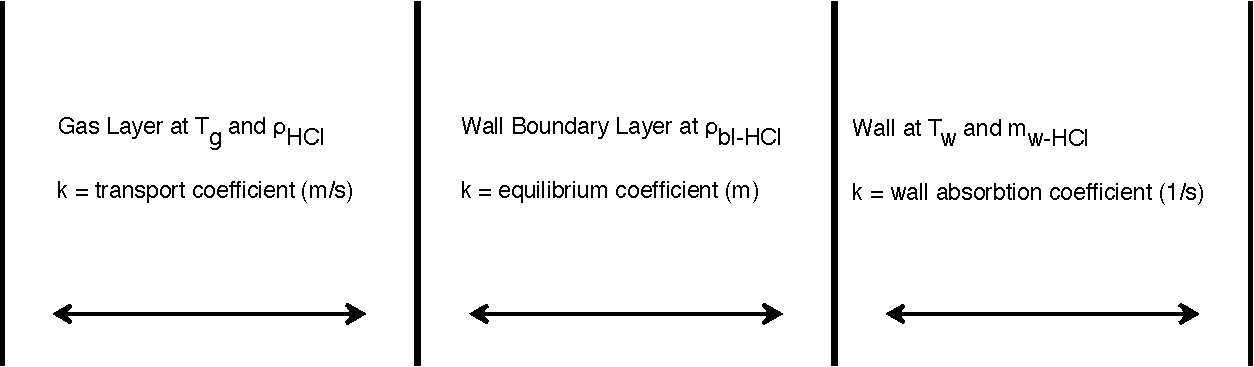
\includegraphics[width=5.0in]{FIGURES/Theory/HCl_Deposition}\\
\end{center}
\caption{Schematic of hydrogen chloride deposition region.}
 \label{fig:HCl_Deposition}
\end{figure}

The rate of addition of mass of hydrogen chloride to the gas layer is given by

\be \frac{d}{dt} m_{HCl} = source - k_c \brackets{\rho_{HCl} - \rho_{bl-HCl}} A_w \ee
where source is the production rate from the burning object plus flow from other compartments. For the wall concentration, the rate of addition is

\be \frac{d}{dt} d_{w-HCl} = k_c \brackets{\rho_{HCl} - \rho_{bl-HCl}} - k_s m_{w-HCl} \ee
where the concentration in the boundary layer, $\rho_{bl-HCl}$  is related to the wall surface concentration by the equilibrium constant $k_e$, by the relation $\rho_{bl-HCl} = d_{w-HCl} / k_e$. We never actually solve for the concentration in the boundary layer, but it is available, as is a boundary layer temperature if it were of interest.  The transfer coefficients are

\be k_c = \frac{\dot{q}}{\Delta T \rho_g c_p} \ee
\be k_e = \frac{b_1 e^{1500/T_w}}{1 + b_2 e^{1500/T_w} \rho_{HCl}} \brackets{1 + \frac{b_5 \brackets{\rho_{H_2O}}^{b_6}}{\brackets{\rho_{H_2O,sat} - \rho_{H_2O,g}}^{b_7}} } \ee
\be k_s = b_3 e^{-\brackets{\frac{b_4}{R T_w}}} \ee

The only values currently available  for these quantities are shown in table \ref{tab:HCL_Deposition} \cite{Galloway:1990}.  The ``$b$'' coefficients are parameters which are found by fitting experimental data to the above equations. These coefficients reproduce the adsorption and absorption of HCl reasonably well.  Note though that error bars for these coefficients have not been reported in the literature.

\begin{table}
\begin{center}
\caption{Transfer coefficients for HCl deposition}
\label{tab:HCL_Deposition}
\begin{tabular}{| c | c | c | c | c | c | c | c |}
\hline
\multirow{2}{*}{Surface} & $b_1$ & $b_2$ & $b_3$ & $b_4$ & $b_5$ & $b_6$ & $b_7$ \\
 & (m) & (m\superscript{3}/kg) & (s\superscript{-1}) & (J/g mol) & (m\superscript{3}/kg)\superscript{$b_7 - b_6$} & (note a) & (note b) \\
 \hline
 Painted Gypsum & 0.0063 & 191.8 & 0.0587 & 7476 & 193 & 1.021 & 0.431 \\ \hline
 PMMA & $9.6 x 10^{-5}$ & 0.0137 & 0.0205 & 7476 & 29 & 1.0 & 0.431 \\ \hline
 Ceiling Tile & $4.0 x 10^{-3}$ & 0.0548 & 0.123 & 7476 & 30\superscript{a} & 1.0 & 0.431 \\ \hline
 Cement Block & $1.8 x 10^{-2}$ & 5.48 & 0.497 & 7476 & 30\superscript{a} & 1.0 & 0.431 \\  \hline
 Calcium Silicate Board & $1.9 x 10^{-2}$ & 0.137 & 0.030 & 7476 & 30\superscript{a} & 1.0 & 0.431 \\  \hline
\end{tabular}
\end{center}
a - very approximate value, insufficient data for high confidence value

b - non-dimensional
\end{table}

The experimental basis for poly(methyl methacrylate) and gypsum cover a sufficiently wide range of conditions that they should be usable in a variety of practical situations.  The parameters for the other surfaces do not have much experimental backing, and so their use should be limited to comparison purposes.

\section{Single Zone Approximation}

A single zone approximation is appropriate for smoke flow far from a fire source where the two-zone layer stratification is less pronounced than in compartments near the fire. In this situation, a single zone approximation may be derived by using the normal two-zone source terms and the substitutions:

\be
\begin{array}{rcl}
\dot{m}_U^{new} &=& \dot{m}_L + \dot{m}_U \\
\dot{m}_L^{new} &=& 0 \\
Q_U^{new} &=& Q_L + Q_U \\
Q_L^{new} &=& 0
\end{array}
\ee

This is used in situations where the stratification does not occur. Examples are elevators shafts, complex stairwells, natural venting ductwork, and compartments far from the fire.

